%%%%%%%%%%%%%%%%%%%%%%%%%%%%%%%%%%%%%%%%%%%%%%%%%%%%%%%%%%%%%%%%%%%%%%
% Problem statement
\begin{statement}[
  problempoints=110,
  timelimit=1 sekunda,
  memorylimit=512 MiB,
]{Zoo}

\setlength\intextsep{-0.1cm}
\begin{wrapfigure}[12]{r}{0.23\textwidth}
\centering

\includegraphics[width=0.23\textwidth]{img/tragovi.png}
\end{wrapfigure}

Kasno uvečer, na Božić 2010., Zdravko je odlučio izaći iz kuće, prijeći cestu te
prošetati snježnim maksimirskim parkom. Nažalost, zimsku je idilu prekinuo jedan
monstrum koji je iskočio iz grma. No, Zdravko se nije prepao, već je odlučio
otjerati monstruma glasnim urlikanjem. Operacija je uspjela, monstrum se
preplašio i pobjegao, a Zdravko je nastavio šetnju parkom ne sluteći da je
njegovo urlikanje uzburkalo dio životinja koje se nalaze u obližnjem zoološkom
vrtu. Preciznije, Zdravkovo urlikanje je najviše uzburkalo tigrove i bikove koji
su odlučili pobjeći iz zoološkog vrta kako bi pronašli mirnije mjesto za
spavanje.

Tijekom bijega, tigrovi i bikovi morali su proći kroz ograđeno, snijegom
prekriveno, pravokutno područje podijeljeno na $R \times S$ jediničnih polja.
Ove životinje u pravokutno su područje morale ući preko gornjeg lijevog kuta, a
iz područja su morale izaći preko donjeg desnog kuta. Kako bi u što većoj tišini
prošle kroz ovo područje, životinje su područjem prolazile jedna po jedna,
krećući se proizvoljnim putem u četiri osnovna smjera (gore, dolje, lijevo,
desno). Odnosno, životinja se tijekom bijega nije nužno kretala najkraćim putem
te je na neka polja (uključivo sa početnim i završnim) mogla stati više puta.
Budući da je pravokutno područje prekriveno snijegom, životinje ostavljaju
tragove kada stanu na neko polje (potencijalno brišući trag prethodne životinje
koja je prošla tim poljem).

Odredite najmanji mogući broj životinja koje su pobjegle iz zoološkog vrta na
temelju ostavljenih tragova na spomenutom pravokutnom području.

%%%%%%%%%%%%%%%%%%%%%%%%%%%%%%%%%%%%%%%%%%%%%%%%%%%%%%%%%%%%%%%%%%%%%%
% Input
\subsection*{Ulazni podaci}
U prvom su retku prirodni brojevi $R$ i $S$ iz teksta zadatka. \\
U sljedećih je $R$ redaka po $S$ znakova koji predstavljaju pravokutno područje
iz teksta zadatka. Znak \texttt{T} označava tigrov trag, znak \texttt{B}
označava bikov trag, a znak \texttt{*} označava netaknuto područje prekriveno
snijegom.

Možete pretpostaviti da su ulazni podaci takvi da je barem jedna životinja ušla
u pravokutno područje i da je svaka takva životinja iz njega i izašla te da se
pritom kretala u skladu s tekstom zadatka.

%%%%%%%%%%%%%%%%%%%%%%%%%%%%%%%%%%%%%%%%%%%%%%%%%%%%%%%%%%%%%%%%%%%%%%
% Output
\subsection*{Izlazni podaci}
U jednom retku ispišite najmanji mogući broj životinja koje su pobjegle iz
zoološkog vrta.

%%%%%%%%%%%%%%%%%%%%%%%%%%%%%%%%%%%%%%%%%%%%%%%%%%%%%%%%%%%%%%%%%%%%%%
% Scoring
\subsection*{Bodovanje}
{\renewcommand{\arraystretch}{1.4}
  \setlength{\tabcolsep}{6pt}
  \begin{tabular}{ccl}
 Podzadatak & Broj bodova & Ograničenja \\ \midrule
    1 & 22 & \makecell[l]{$2 \le R, S \le 100$ \\ Na sva će polja osim početnog
    i završnog (ne nužno jednom) \\ stati najviše jedna životinja.} \\
  2 & 33 & $2 \le R, S \le 100$ \\
  3 & 55 & $2 \le R, S \le 1000$ \\
\end{tabular}}

%%%%%%%%%%%%%%%%%%%%%%%%%%%%%%%%%%%%%%%%%%%%%%%%%%%%%%%%%%%%%%%%%%%%%%
% Examples
\subsection*{Probni primjeri}
\begin{tabularx}{\textwidth}{X'X'X}
\sampleinputs{test/zoo.dummy.in.1}{test/zoo.dummy.out.1} &
\sampleinputs{test/zoo.dummy.in.2}{test/zoo.dummy.out.2} &
\sampleinputs{test/zoo.dummy.in.3}{test/zoo.dummy.out.3}
\end{tabularx}

\textbf{Pojašnjenje drugog probnog primjera:}

\begin{wrapfigure}{c}{\textwidth}
\centering
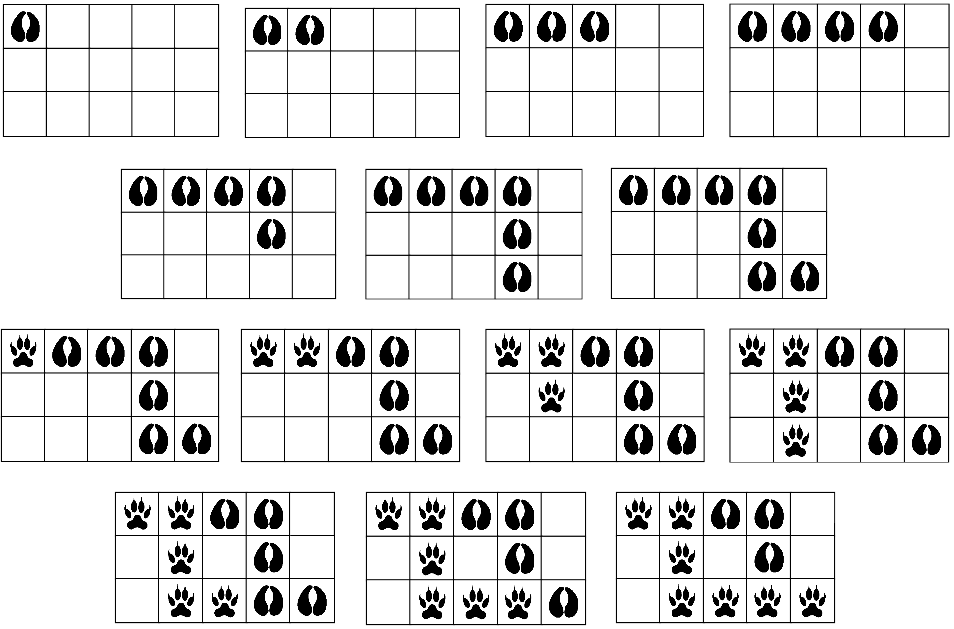
\includegraphics[width=\textwidth]{img/escape.png}
\end{wrapfigure}


%\textbf{1. upit} \textrightarrow{}
%$A_9 = 9$, $A_{10} = 1 + 0 = 1$, $A_{11} = 1 + 1 = 2$,
%$A_{12} = 1 + 2 = 3$, $A_{13} = 1 + 3 = 4$.\\
%\phantom{\textbf{1. upit} \textrightarrow{}}
%$A_9 + A_{10} + A_{11} + A_{12} + A_{13} = 9 + 1 + 2 + 3 + 4 = 19$.

%\textbf{2. upit} \textrightarrow{}
%$A_{44} = 4 + 4 = 8$, $A_{45} = 4 + 5 = 9$. $A_{44} + A_{45} = 8 + 9 = 17$.

%%%%%%%%%%%%%%%%%%%%%%%%%%%%%%%%%%%%%%%%%%%%%%%%%%%%%%%%%%%%%%%%%%%%%%
% We're done
\end{statement}

%%% Local Variables:
%%% mode: latex
%%% mode: flyspell
%%% ispell-local-dictionary: "croatian"
%%% TeX-master: "../hio.tex"
%%% End:
